\section{Applications}

\subsection{Compas dataset}
\begin{frame}{Compas dataset}
    \begin{columns}
        \begin{column}{0.65\textwidth}
        \begin{itemize}
            \item The \gbf{COMPAS dataset} contains information about \gbf{defendants} and their \gbf{criminal history}.
            \item The goal is to predict whether a defendant will \gbf{re-offend}.
            \item It has been shown that the COMPAS algorithm is \gbf{biased against certain demographic populations} like African-Americans even though ethnicity was not included in the features.
        \end{itemize}
        \end{column}
        \begin{column}{0.35\textwidth}
        \begin{figure}
            \centering
            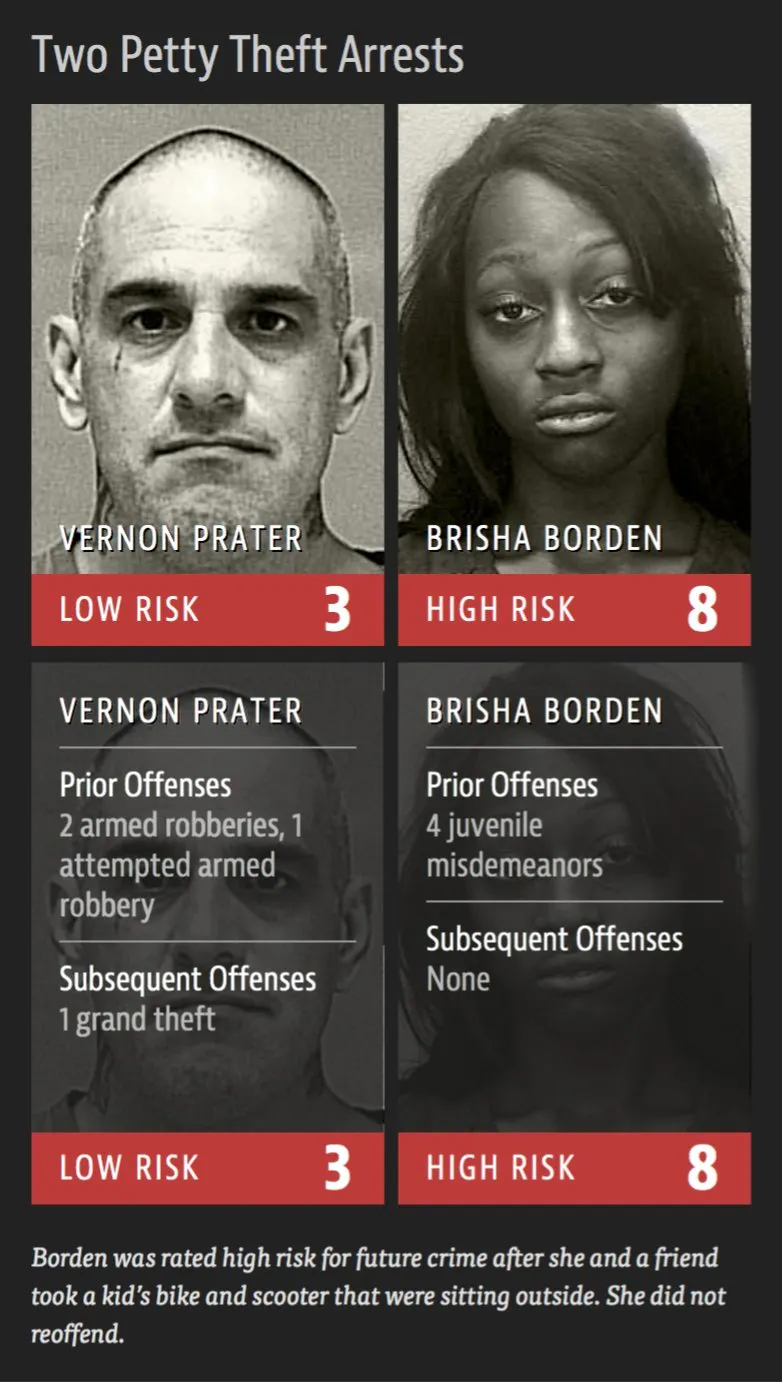
\includegraphics[width=0.9\columnwidth]{images/compas.png}
            \caption{Bias from the COMPAS Algorithm}
            \label{fig:compas_dataset}
        \end{figure}
        \end{column}
    \end{columns}
    
\end{frame}

\subsection{Adult dataset}
\begin{frame}{Adult dataset}
        \begin{itemize}
            \item The \gbf{Adult dataset} contains information about \gbf{individuals} and their \gbf{income}.
            \item The goal is to predict whether an individual earns more than \$50,000 a year.
            \item It has been shown that the Adult dataset is \gbf{biased against women}.
        \end{itemize}
\end{frame}

\subsection{Results}
\begin{frame}{Results}
    \begin{figure}
        \centering
        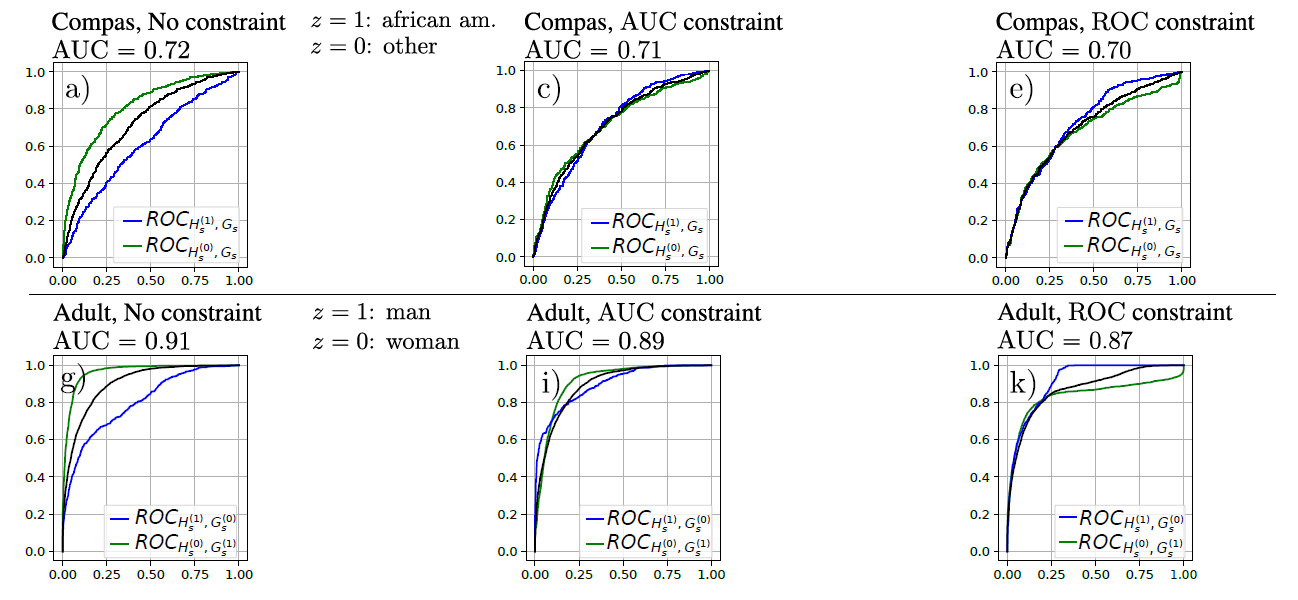
\includegraphics[width=\textwidth]{images/resultsmodified.png}
            \caption{$ROC$ curves on the test set of Adult and Compas
            for a score learned without and with fairness constraints.
            Black curves represent $ROC_{H_s,G_s}$.}
            \label{fig:roc_real_main_text}
    \end{figure}
        
\end{frame}
